
% !TEX encoding = UTF-8 Unicode

\documentclass[a4paper]{report}

\usepackage[francais]{babel}
\usepackage[T1]{fontenc}
\usepackage[utf8]{inputenc}
\usepackage{geometry}
\usepackage{graphicx}
\usepackage[colorlinks=true]{hyperref}
%\usepackage{algorithm,algorithmic}
\usepackage{listings}
\usepackage{amssymb}
\usepackage{setspace}
\usepackage{listings}
\usepackage{lscape}
%\usepackage{mathabx}
\usepackage{amsmath}
\usepackage{mathrsfs}
\usepackage{amsthm}
\usepackage{textcomp}
\usepackage{enumerate}
\usepackage{tikz}
\usepackage{verbatim} 

\hypersetup{urlcolor=blue,linkcolor=black,citecolor=black,colorlinks=true}
\geometry{a4paper,twoside,left=2.5cm,right=2.5cm,marginparwidth=1.2cm,marginparsep=3mm,top=2.5cm,bottom=2.5cm}
\setlength{\parskip}{5mm plus2mm minus2mm}
\lstset{language=C, showstringspaces=false, numbers=left, numberstyle=\tiny, tabsize=4}

\theoremstyle{definition}
\newtheorem{mydef}{D\'efinition}
\newtheorem{mylem}{Lemme}



\begin{document}
\normalsize
\pagenumbering{arabic}

%\maketitle

\begin{titlepage}

\begin{minipage}[c][4cm][t]{7.8cm}
\raggedright 

\includegraphics[width=6cm]{./logo_um2}
\end{minipage}
\begin{minipage}[c][4cm][t]{7.8cm}
\raggedleft

\includegraphics[width=6cm]{./LogoLIRMM}
\end{minipage}

\vfill

\begin{center}
\textsc{\Large SQR M1 Informatique}\\[0.5cm]

\hspace{0.4cm}
{ \huge \bfseries Travaux pratiques de Services et Qualité Reseaux}\\[3cm]

\begin{minipage}[c][4cm][t]{0.4\textwidth}
\raggedright \large
\emph{Auteurs:}\\
Rabah LAOUADI\\
Samuel ROUQUIE
\end{minipage}

\vfill
{\large  Avril 2012}
\end{center}
\end{titlepage}

\chapter*{TP1: Simulation de reseaux IP avec NS}
\section*{Objectifs}Se familiariser avec le logiciel de simulation ns et ses outils périphériques. 
Réaliser une étude du protocole TCP: mesurer des débits et des taux de perte, étudier l'evolution des fenêtres du protocols TCP, étudier l'influence de différents paramètres.
\section*{Topologie du reseau} 

Le réseau comprend une paire de noeuds $(O,D)$ par lesquels vont passer quatre trafics de $O$ à $D$:trois TCP et un UDP. La capacité du lien $(O,D)$ est de $2 Mb/s$ et sa latence $20 ms$.La capacité de la file d'atttente de $D$ est 
de 100 paquets et la discipline est Droptail. 
\begin{enumerate}
 \item Le trafic UDP suit une loi exponentiel. La durée moyenne des périodes $on$ et $off$ sont respectivement de 10 et 5 $ms$.
 \item Les trafics TCP sont de débits constant (CBR) . La latence totale pour les différents trafics est 50 $ms$, 100 $ms$ et 150 $ms$.
\end{enumerate}

%Fugure 1
\begin{center}

	\begin{figure}[h]
	\centering
		\begin{tikzpicture}[auto,node distance=1.5cm,  semithick]
		 \tikzstyle{every node}=[draw,shape=circle,fill=white,minimum size=15pt, inner sep=0pt]
	
		  \node         (0)   		     {O};
  		  \node         (1) [ right of=0]    {D};

		  \path(0) edge  (1);
		\end{tikzpicture}
		\caption{Topologie du reseau}
	\end{figure}
\end{center}

\section*{Code::Script}
 Tout le code source est écrit en NS (TCL), et toutes les courbes sont générées à partir de ce script.
\begin{verbatim} 
set ns [new Simulator]

$ns color 0 blue
$ns color 1 red
$ns color 2 black
$ns color 3 green

set n0 [$ns node]
set n1 [$ns node]

set FQ  [open filAtt.tr w]
set f [open out.tr w]
$ns trace-all $f
set nf [open out.nam w]
$ns namtrace-all $nf

$ns duplex-link $n0 $n1 2Mb 20ms DropTail

set spy [$ns monitor-queue $n0 $n1 $FQ]

#UDP
set udp0 [new Agent/UDP]
$ns attach-agent $n0 $udp0
$udp0 set class_ 3

set null0 [new Agent/Null]
$ns attach-agent $n1 $null0

$ns connect $udp0 $null0


#TCPS
set tcp0 [new Agent/TCP]
$ns attach-agent $n0 $tcp0
$tcp0 set class_ 0


set tcp1 [new Agent/TCP]
$ns attach-agent $n0 $tcp1
$tcp1 set class_ 1

set tcp2 [new Agent/TCP]
$ns attach-agent $n0 $tcp2
$tcp2 set class_ 2

set sink0 [new Agent/TCPSink]
$ns attach-agent $n1 $sink0

set sink1 [new Agent/TCPSink]
$ns attach-agent $n1 $sink1

set sink2 [new Agent/TCPSink]
$ns attach-agent $n1 $sink2

$ns connect $tcp0 $sink0
$ns connect $tcp1 $sink1
$ns connect $tcp2 $sink2


#applications
set cbr0 [new Application/Traffic/CBR]
$cbr0 set paquetsSize_ 20936	
$cbr0 set interval_ 50ms		
$cbr0 attach-agent $tcp0

set cbr1 [new Application/Traffic/CBR]
$cbr1 set paquetsSize_ 41872
$cbr1 set interval_ 100ms
$cbr1 attach-agent $tcp1
	
set cbr2 [new Application/Traffic/CBR]
$cbr2 set paquetsSize_ 62808
$cbr2 set interval_ 150ms
$cbr2 attach-agent $tcp2

set cbr3 [new Application/Traffic/Exponential]
$cbr3 set rate_ 2Mb
$cbr3 set burst_time_ 100ms
$cbr3 set idle_time_ 100ms
$cbr3 attach-agent $udp0


$ns at 0.1 "$cbr0 start"
$ns at 0.1 "$cbr1 start"
$ns at 0.1 "$cbr2 start"
$ns at 0.1 "$cbr3 start"

$ns at 10.0 "finish"
$ns at 0.2 "tailleTcp"
#FILE aTTENT + Window
$ns queue-limit $n0 $n1 100
#$tcp0 set window_ 10
#$tcp1 set window_ 10
#$tcp2 set window_ 10

#Statistiques
#TCP FenaitreTAILLE des fenêtre
set delaiTcp 0.01

proc tailleTcp {} {
	global ns delaiTcp tcp0 tcp1 tcp2
	set now [$ns now]
	set newAt [expr $now + $delaiTcp]  

	puts "TCP0 a l'instant $now [$tcp0 set cwnd_]"
	$ns at  $newAt "tailleTcp"
}

#Monitor TCPs
$tcp0 set fid_ 0
$tcp1 set fid_ 1
$tcp2 set fid_ 2
$udp0 set fid_ 3

set flowtcp0 [$ns makeflowmon Fid]
set link0 [$ns link $n0 $n1]
$ns attach-fmon $link0 $flowtcp0
set fcl [$flowtcp0 classifier]


#FILE d'attent
set delaiFile 0.01
set tcpF0 [open tcp0.tr w]
set tcpF1 [open tcp1.tr w]
set tcpF2 [open tcp2.tr w]

proc tailleTcp {} {
	global ns delaiFile tcpF0 tcpF1 tcpF2 tcp0 tcp1 tcp2 FQ spy
	set now [$ns now]
	set newAt [expr $now + $delaiFile]  

#TAILLE des FENEAITRE
	puts $tcpF0  	"0 $now [$tcp0 set cwnd_]"
	puts $tcpF1 	"1 $now [$tcp1 set cwnd_]"
	puts $tcpF2 	"2 $now [$tcp2 set cwnd_]"
        puts $FQ	"$now [$spy set pkts_ ]"
	$ns at  $newAt "tailleTcp"
}


proc finish {} {
	global ns f nf cbr0 cbr1 cbr2 cbr3 spy fcl tcp0 tcp1 tcp2
	$ns flush-trace
	close $f
	close $nf

	puts "Def Max Windows [$tcp0 set window_ ]"
	#puts "ON def [$cbr3 set burst_time_]"
	#puts "OFF def [$cbr3 set idle_time_]"
	#puts "paquets size defalt [$cbr2 set paquetsSize_]"
	#puts "interval default [$cbr2 set interval_]"
	#puts "rate default [$cbr2 set rate_]"

	puts "LES PARAMAITRE  INITIALs"
	puts "paquets CBR0  [$cbr0 set paquetsSize_]\t-Interval\t[$cbr0 set interval_]"
	puts "paquets CBR1  [$cbr1 set paquetsSize_]\t-Interval\t[$cbr1 set interval_]"
	puts "paquets CBR2  [$cbr2 set paquetsSize_]\t-Interval\t[$cbr2 set interval_]"
	puts "paquets EXP   [$cbr3 set paquetsSize_]\t-Rate \t\t[$cbr3 set rate_]"


	puts "\n Les PARAMAITRES de SORTIe"
	puts "Les paquetss"

	puts "paquets envoyer [$spy set pdepartures_]"
	puts "paquets recus [$spy set parrivals_]"
	puts "paquets droped [$spy set pdrops_]"
	puts "Le taux de perte globale [expr [format %f [$spy set pdrops_]]/[format %f [$spy set
	 pdepartures_]]]"


	puts "\n débit Moyenne"
	puts "nombre de octets envoyer [$spy set bdepartures_]"
	puts "le temps de Simulation est de [$ns now] s"
	puts "le débit crete est de 250000 octets/s"
	puts "le débit moyen est de  [expr [format %f [$spy set bdepartures_]]/[format %f [$ns
	 now]]]  octets/s"


	set stats_tcp0 [$fcl lookup auto 0 0 0]
	
	puts "\n PARAMAITRE dechaque TCP"
	puts "TCP0:"
	#puts "paquets envoyer [$stats_tcp0 set pdepartures_]"
	#puts "paquets recus [$stats_tcp0 set parrivals_]"
	#puts "paquets droped [$stats_tcp0 set pdrops_]"
	puts "TCP Le taux de perte [expr [format %f [$stats_tcp0 set pdrops_]]/[format %f
	 [$stats_tcp0 set pdepartures_]]]"
	puts "le débit moyen est de  [expr [format %f [$stats_tcp0 set bdepartures_]]/[format %f
	 [$ns now]]]  octets/s"


	set stats_tcp1 [$fcl lookup auto 0 0 1]
	puts "\nTCP1:"
	#puts "paquets envoyer [$stats_tcp1 set pdepartures_]"
	#puts "paquets recus [$stats_tcp1 set parrivals_]"
	#puts "paquets droped [$stats_tcp1 set pdrops_]"
	puts "TCP Le taux de perte [expr [format %f [$stats_tcp1 set pdrops_]]/[format %f
	 [$stats_tcp1 set pdepartures_]]]"
	puts "le débit moyen est de  [expr [format %f [$stats_tcp1 set bdepartures_]]/[format %f
	 [$ns now]]]  octets/s"

	set stats_tcp2 [$fcl lookup auto 0 0 2]
	puts "\nTCP2:"
	#puts "paquets envoyer [$stats_tcp2 set pdepartures_]"
	#puts "paquets recus [$stats_tcp2 set parrivals_]"
	#puts "paquets droped [$stats_tcp2 set pdrops_]"
	puts "TCP Le taux de perte [expr [format %f [$stats_tcp2 set pdrops_]]/[format %f
	 [$stats_tcp2 set pdepartures_]]]"
	puts "le débit moyen est de  [expr [format %f [$stats_tcp2 set bdepartures_]]/[format %f 
	 [$ns now]]]  octets/s"

	
	set stats_udp [$fcl lookup auto 0 0 3]
	puts "\nUDP:"
	#puts "paquets envoyer [$stats_udp set pdepartures_]"
	#puts "paquets recus [$stats_udp set parrivals_]"
	#puts "paquets droped [$stats_udp set pdrops_]"
	puts "TCP Le taux de perte [expr [format %f [$stats_udp set pdrops_]]/[format %f
	 [$stats_udp set pdepartures_]]]"
	puts "le débit moyen est de  [expr [format %f [$stats_udp set bdepartures_]]/[format %f
	 [$ns now]]]  octets/s"


    	exit 0
}

$ns run	
\end{verbatim} 

\section*{Résultats}
	Avant de commencer les différents simulations, nous allons étudier le cas par default, aprés nous verrons l'influence des différents paramètres sur le taux de perte ainsi d'étudier la formule de la question 3, et pour cela nous avons un tableau contenant les résultats obtenu à partir de la simulation et celle que nous avons obtenu de l'equation   :
\subsection*{Paramètres par default:}
	Dans le premier Cas,  Nous allons examiner les paramétres utilisés par NS2 sur les flux TCPs.\\
	le tableaux suivant représente les paramétres utilisés par NS2: 
\begin{center}
\begin{tabular}{|c|c|}
\hline
 paramètre  & valeur \\ \hline
 
 Capacité de lien (Mbit/s) & 2 \\ 
 Capacité en (o/s)  & 250000 \\ 
 Rate (Mbit/s) & 1.5 \\ 
 ON & 0.01\\ 
 OFF & 0.01 \\ 
 Max Window  & pas de Max\\ 
 Taille File d'attente & 100\\
\hline
\end{tabular}\\
\end{center}

les résultats obtenus avec ces paramètres dans les deux cas: avec la fonction et avec la simulations :\\
\begin{center}

\begin{tabular}{|l|c|c|c|c|c|c|c|}
\hline
 IdTCP & Taux Perte & Latence & T paquets(Octet) & T Packat(bits) & Débit Moy.(O/S) & DM(bits/S) \\ \hline
 0 & 0.0800 & 0.00375 & 1024 & 8192 & 250000 & 966190.70\\
 1 & 0,0695 & 0.00375 & 1024 & 8192 & 250000 & 1035887,49\\ 
 2 & 0,0784 & 0.00375 & 1024 & 8192 & 250000 & 975951,95\\ \hline
 final & \multicolumn{2}{c|}{Débit moyenne Obtenu} & en Octect/S & 247067 & en bits/S & 1976536 \\ 
\hline
\end{tabular}
\end{center}
\paragraph*{} D'aprés le tableau, Nous remarquons que le débit des trois flux TCP converge ver 1Mbit, ce qui est confirmé dans l'énoncé de ce TP, par contre le résultats prédis par la formule (1) est superieur au débit maximal, et cela est due a la grande perte des paquets. 
\subsection*{Les modification selon l'ennoncé de TP:}
\paragraph{}
	Dans le deuxieme Cas, nous allons voir les resultâts obtenus avec l'utilisation des paramétres de l'enoncé de TP, et nous allons garder les mêmes taux de pertes, ainsi les débit obtenu avec le changemant de la latence de TCP1, TCP2 et TCP3 a 0.050s, 0.100s et 0.150s respectivement, et cela a l'aide de la formule vue en cours.\\
	Afin de garder les mêmes taux de pertes, nous somme dans l'obligation de changer les tailles des paquetss d'applications des flux TCPs.\\
	le tableau suivant représente les paramétres utilisés pour cette simulation:
\begin{center}
\begin{tabular}{|c|c|}
\hline
 paramètre  & valeur \\ \hline
 
 Capacité de lien & 2Mbit/s(250000 o/s) \\ 
 Rate (Mbit/s) & 1.5 \\ 
 ON & 0.01\\ 
 OFF & 0.005 \\ 
 Taille file d'att. & 100\\
\hline
\end{tabular}
\begin{tabular}{|c|c|c|}
\hline
 IdTCP  & Latence(s) & Taille de paquet (O) \\ \hline
 
 0 & 0.050 & 20936 b ( 2617 o)	 \\ 
 1 & 0.100 & 41872 b ( 5234 o)	 \\ 
 2 & 0.150 & 62808 b ( 7851 o)	 \\ 
 - & taille fene. & par default\\ 
 &&\\
 
\hline
\end{tabular}\newline

les résultats obtenus avec les paramètres de TP(la modifications des Flux TCPs, sans touché à UDP): \\ 

\begin{tabular}{|l|c|c|c|c|c|c|c|}
\hline
 protocole & Taux Perte & Débit Moy.(O/S) Théorique & en Simulation (O/S) \\ \hline
 TCP0 & 0,0800 &  903043,24 &  38900     \\
 TCP1 & 0,0608 & 1035861,64 &  46076     \\ 
 TCP2 & 0,0770 &  919929,43 &  47116     \\ 
 UDP  & 0,0831 & 1875000 & 114975 \\ 
 \hline
 final perte & 0.0810  & Somme débit Moy. Sim. & 247067   \\ 
\hline

\end{tabular}
\end{center}
\paragraph*{} Dans ce tableaux où le taux de perte est de 0.810 on moyenne (présque la meme perte pour tous les Flux TCPs ainsi L'UDP) et une correspendance entre le débit calculé à partir de la formule et celui obtenu dans la simulation ou L'UDP qui utilise la grande partie de Débit, et le reste partagé equitablement entre les autres TCPs.
  
\paragraph*{} La courbe suivante représente la taille de La file d'attente ainsi que les fenêtres TCP en fonction de temps de Simulations : \\
%Figures 
\begin{figure}[h]
	\centering
		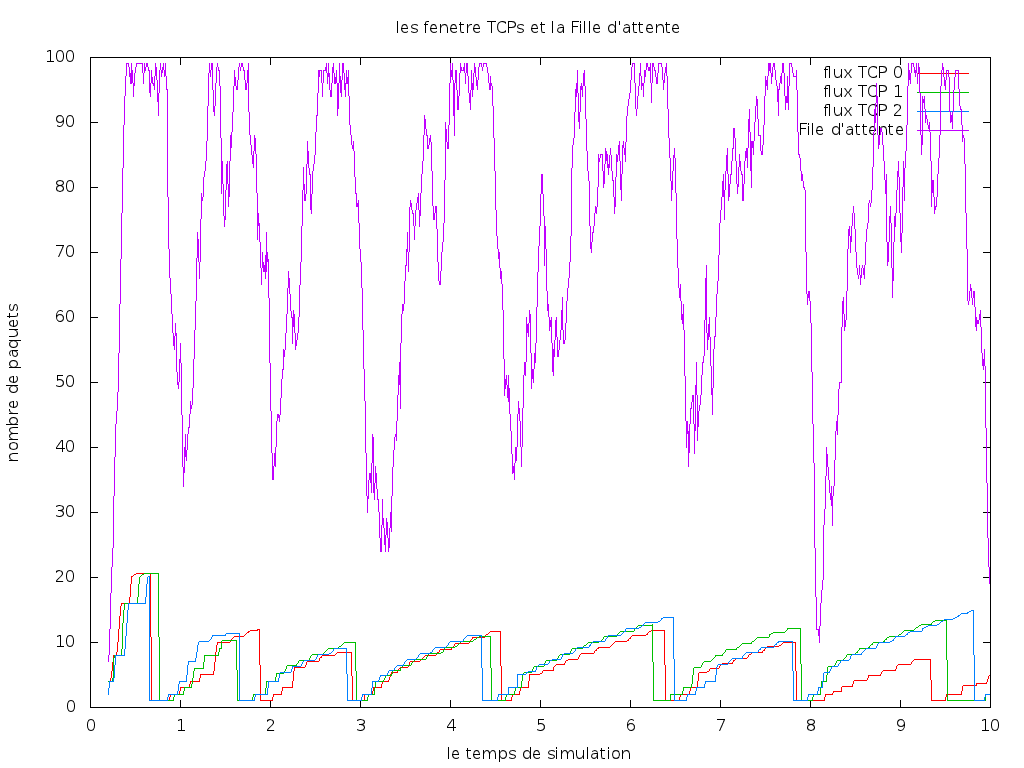
\includegraphics[width=450px]{graphic/tp.png}
		\caption{les Tailles des fenêtre TCPs et la Fille d'attente}
\end{figure}

\paragraph*{} Nous ramarquons qu'il ya une relation d'ordre entre Les tailles des fenêtres TCPs et Le Nombre de paquet dans la fille d'attente, où a chaque fois les tailles de fenêtres augmente, la fille d'attente augmente aussi et vis-versa.\\

      Et pour bien étudier cette relation, nous allons modifier c'est deux paramètres a fin que nous  puissions preuver cette relation, ainsi de voir le comportement de taux de perte au fonction des valeurs de ces deux paramètres.   

\newpage
%%%%%%%%%%%%%%%%%%%%%%%%%%%%%%%%%%%%%%%%%%%%%%%%%%%%%%%%%%%%%%%%%%%%%%%%%%%%%%%%%%%%%%%
\subsection*{File d'attente et les fenêtres TCPs :}
\paragraph{}
    Dans cette partie, Nous allons étudier les deux paramétres: la file d'attente et la fenêtre TCP.
	Pourquoi file d'attente et la fenêtre TCP, parce qu'ils ya une liaison direct entre ces deux paramétres d'aprés la courbe précédemment obtenu, et aussi parce que la fenêtre TCP qui est Congestion des paquets dans la file TCP depend de la Taille de la fille d'attente globale.
\subsubsection{File d'attente :}
\paragraph*{}
   Nous allons commencer par la modification de la valeur de la file d'attente, l'augmenté a 200 paquets pour commencé afin de vérfier l'influance de ce paramétre sur le taux de perte, les fenêtre TCPs, ainsi la simulation.\\
	Les paramétres utilisé pour cette simulations: \\
	\begin{center}
	

\begin{tabular}{|c|c|}
\hline
 paramètre  & valeur \\ \hline
 
 Capacité de lien & 2Mbit/s(250000 o/s) \\ 
 Rate (Mbit/s) & 1.5 \\ 
 ON & 0.01\\ 
 OFF & 0.005 \\ 
 Taille file d'att. & 200\\
\hline
\end{tabular}
\begin{tabular}{|c|c|c|}
\hline
 IdTCP  & Latence(s) & Taille de paquet (O) \\ \hline
 
 0 & 0.050 & 20936 b ( 2617 o)	 \\ 
 1 & 0.100 & 41872 b ( 5234 o)	 \\ 
 2 & 0.150 & 62808 b ( 7851 o)	 \\ 
 - & taille fene. & 20\\ 
 &&\\
\hline
\end{tabular}\\
	\end{center}
les résultats obtenu avec avec ces paramètres à partir de la simulation et de la formule :  \\

\begin{tabular}{|l|c|c|c|c|c|c|c|}
\hline
 protocole & Taux Perte & Débit Moy.(O/S) Théorique & en Simulation (O/S) \\ \hline
 TCP0 & 0,029 &  187484,14 &  42852     \\
 TCP1 & 0,018 &  234734,91 &  44932     \\ 
 TCP2 & 0,038 &  164434,47 &  41292     \\ 
 UDP  & 0,035 &  187500    &  118041 \\ 
 \hline
 final perte & 0.034  & débit Moy. Sim. & 2471177   \\ 
\hline

\end{tabular}
\paragraph{} Nous remarquons que le taux de perte est de 0.034, qui repressente une grande diminuation par rapport au deux premiéres simulations où le taux de perte etait a 0.081, ce qui prouve que la taille de file d'attente a une infliance majeur sur le taux de perte ainsi que le simulation.
        La relation entre la file d'attente et le taux de perte est une relation inversé, c'est à dir : la taille de la file d'attente augmente, le taux de perte diminue et vis-versa.
	
	la courbe suivante représente comme la premiére la taille de la fille d'attente, ainsi que les fenêtres TCPs en fonction de temps de simulations:
\newpage
\begin{center}

%Figures 
\begin{figure}[h]
	\centering
		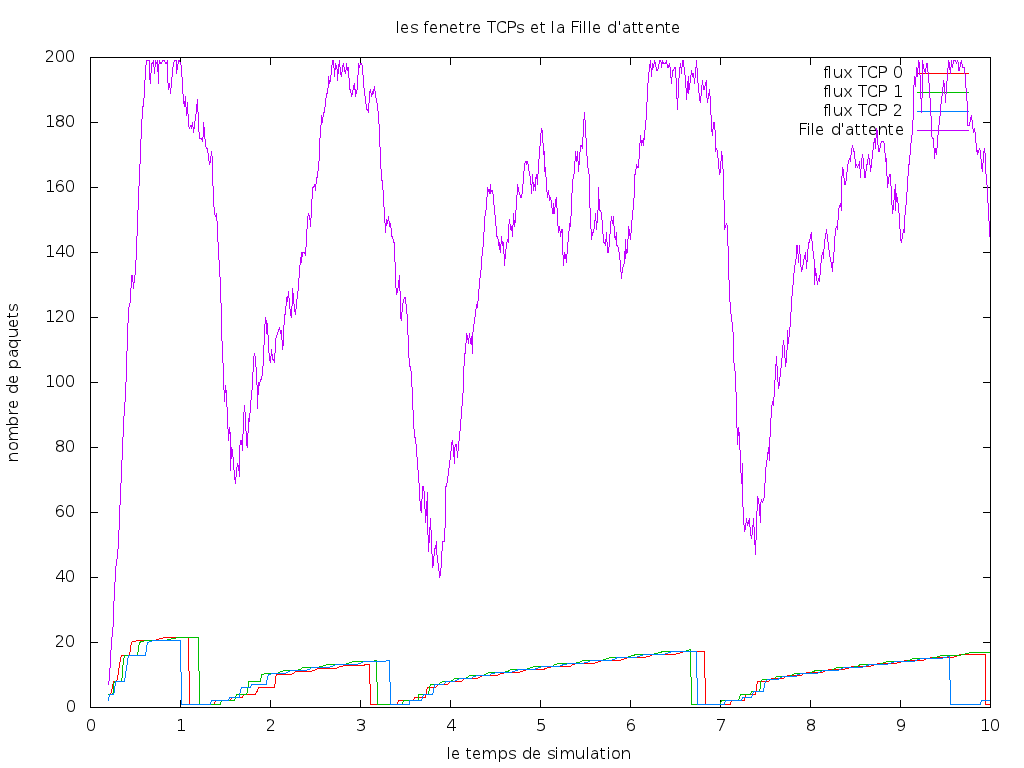
\includegraphics[width=450px]{graphic/f200w20.png}
		\caption{File d'attente = 200}
\end{figure}
\end{center}
	La courbe suivante confirme l'hypothèse de liaison entre la taille de la file d'attente et les tailles des fenêtres TCPs, car nous remarquons que la courbe et plus stable, ce qui diminue la congestion des paquets TCPs.          

%%%%%%%%%%%%%%%%%%%%%%%%%%%%%%%%%%%%%%%%%%%%%%%%%%%%%%%%%%%%%%%%%%%%%%%%%%%%%%%%%%


\subsubsection*{La taille des fenêtres TCPs :}
\paragraph*{}
   Nous allons maintenant étudier l'influance des tailles des fenêtres TCPs sur le taux de perte ainsi, la courbe généré. Et pour cela nous allons diminuer les taille de la fenêtre de chaque TCP  des  En deuxieme cas on diminue la taille de la fenêtre en gardant la file d'attente à 10 avec comme file d'attente maximale de 100 paquets.\\  
   Les deux tableaux suivants représentent les paremètres utilisés dans la simulation sur NS2:
   \begin{center}
   

\begin{tabular}{|c|c|}
\hline
 paramètre  & valeur \\ \hline
 
 Capacité de lien & 2Mbit/s(250000 o/s) \\ 
 Rate (Mbit/s) & 1.5 \\ 
 ON & 0.01\\ 
 OFF & 0.005 \\ 
 Taille file d'att. & 100\\
\hline
\end{tabular}
\begin{tabular}{|c|c|c|}
\hline
 IdTCP  & Latence(s) & Taille de paquets (O) \\ \hline
 
 0 & 0.050 & 20936 b ( 2617 o)	 \\ 
 1 & 0.100 & 41872 b ( 5234 o)	 \\ 
 2 & 0.150 & 62808 b ( 7851 o)	 \\ 
 - & taille fene. & 10\\ 
 & & \\
 
\hline
\end{tabular}\\
   \end{center}
les résultats obtenus avec ces paramètres dans la simulation et à partir de la formule : \\

\begin{tabular}{|l|c|c|c|c|c|c|c|}
\hline
 protocole & Taux Perte & Débit Moy.(O/S) Théorique & en Simulation (O/S) \\ \hline
 TCP0 & 0,047 &  146338,99 &  39212     \\
 TCP1 & 0,043 &  154507,51 &  42684     \\ 
 TCP2 & 0,029 &  186840,98 &  46180     \\ 
 UDP  & 0,052 &  187500    &  117999    \\ 
 \hline
 final perte & 0.0496  & débit Moy. Sim. & 246075   \\ 
\hline
\end{tabular}
\paragraph*{}
   Nous remarquons une diminution de taux de perte, ce qui preuve l'influance de ce paramétre sur la simulations.
   La courbe suivante qui représente le taille de la fille d'attente et les fenêtres TCPs en fonction de temps de simulations:
   \begin{center}
   
  
%Figures 
\begin{figure}[h]
	\centering
		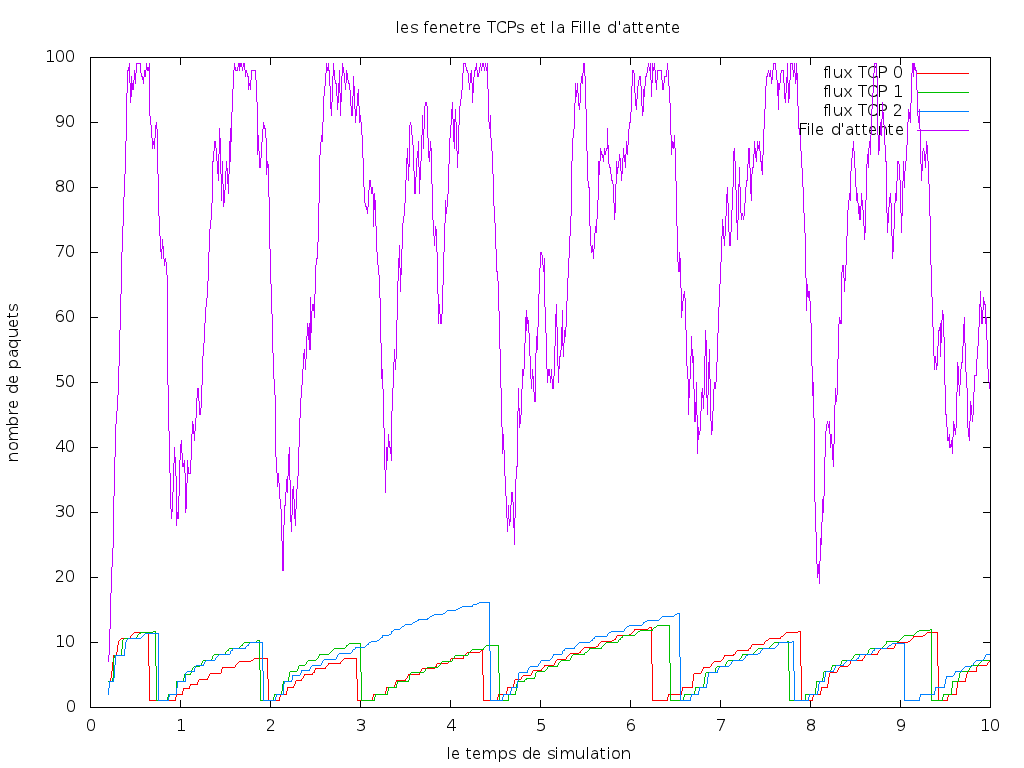
\includegraphics[width=450px]{graphic/f100w10.png}
		\caption{La taille de la fenêtre TCP = 10}
\end{figure}
   \end{center}
   
   Dans cette courbe, nous constatons la relation entre la taille de la file d'attente la taille des fenêtres TCPs.


%%%%%%%%%%%%%%%%%%%%%%%%%%%%%%%%%%%%%%%%%%%%%%%%%%%%%%%%%%%%%%%%%%%
%%%%%%%%%%%%%%%%%%%%%%%%%%%%%%%%%%%%%%%%%%%%%%%%%%%%%%%%%%%%%%%%%%
\subsubsection*{La taille de la fenêtre  et la taille de la fenêtre:}
\paragraph*{}
   Dans le dernier cas de cette sections, nous étudierons l'influance des deux paramètres sur le taux de perte, et aussi sur les résultats de simulation. \\
   Le tableaux suivant représente les parmaitre choisi dans la simulation de NS, où la diminution de la taille de la file d'attente à 50, et la taille des fenêtres TCPs à 10:\\    
   \begin{center}
   

\begin{tabular}{|c|c|}
\hline
 paramètre  & valeur \\ \hline
 
 Capacité de lien & 2Mbit/s(250000 o/s) \\ 
 Rate (Mbit/s) & 1.5 \\ 
 ON & 0.01\\ 
 OFF & 0.005 \\ 
 Taille file d'att. & 50\\
 
\hline
\end{tabular}
\begin{tabular}{|c|c|c|}
\hline
 IdTCP  & Latence(s) & Taille de paquet (O) \\ \hline
 
 0 & 0.050 & 20936 b ( 2617 o)	 \\ 
 1 & 0.100 & 41872 b ( 5234 o)	 \\ 
 2 & 0.150 & 62808 b ( 7851 o)	 \\ 
 - & taille fene. & 10\\ 
 &&\\
 
\hline
\end{tabular}\\
   \end{center}
les résultats obtenu avec ces paramètres à partir de la simulation et de formule    \\
\begin{center}


\begin{tabular}{|l|c|c|c|c|c|c|c|}
\hline
 protocole & Taux Perte & Débit Moy.(O/S) Théorique & en Simulation (O/S) \\ \hline
 TCP0 & 0,084 &  110159,99 &  41812     \\
 TCP1 & 0,089 &  107020,88 &  39316     \\ 
 TCP2 & 0,042 &  155789,75 &  51068     \\ 
 UDP  & 0,084 &  187500    &  114849    \\ 
 \hline
 final perte & 0.081  & débit Moy. Sim. & 247045   \\ 
\hline
\end{tabular}
\end{center}
Nous constatons que le taux de perte est présque la meme valeur que la simulation de l'énoncé de TP, ce qui nous donne une relation d'ordre entre ces deux paramètres et le taux de perte globale. 
	La courbe suivante représente la taille de la file d'attente en fonction de temps de simulation: 
%Figures 
\begin{figure}[h]
	\centering
		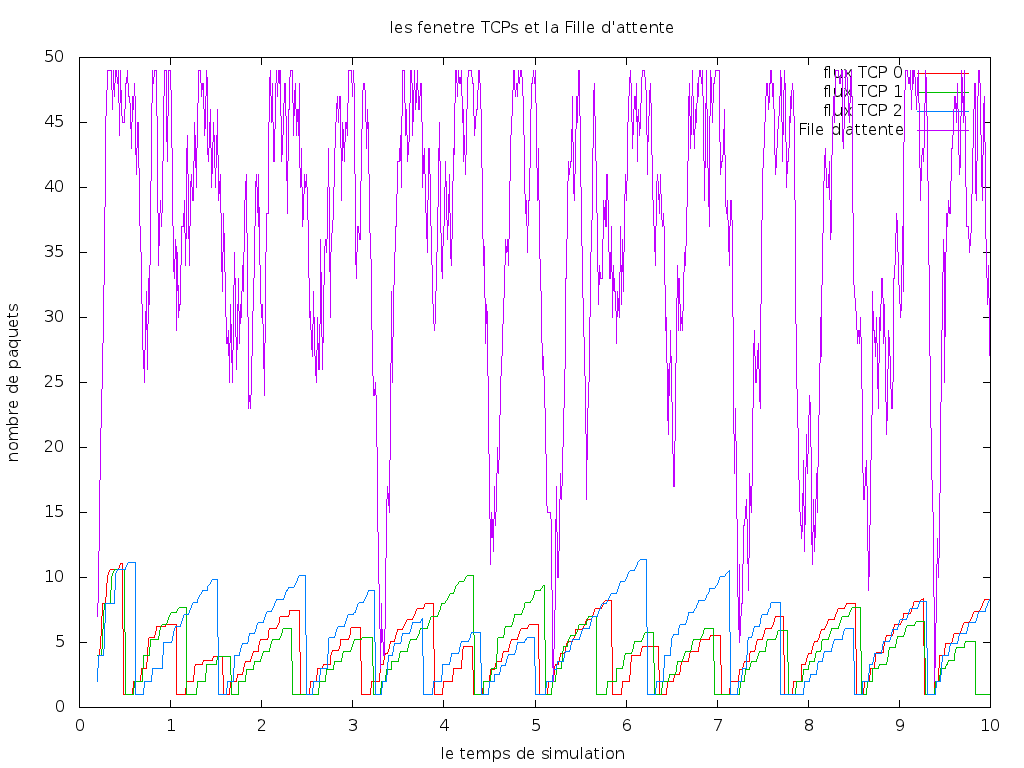
\includegraphics[width=450px]{graphic/f50w10.png}
		\caption{File d'attente = 50, la taille de fenêtre 10}
\end{figure}
Nous remarquons une courbe avec une forte varité due a la diminution des deux paramètres (file d'attente, fenêtre TCPs).\\
Apres avoir etudier les différents cas de la taille de la fille d'attente et celle des fenêtres TCPs, nous allons passer maintenant au flux UDP, pour voir son influance sur le taux de perte.

\newpage
%%%%%%%%%%%%%%%%%%%%%%%%%%%%%%%%%%%%%%%%%%%%%%%%%%%%%%%%%%%%%%%%%%%%%%%%
%%%%%%%%%%%%%%%%%%%%%%%%%%%%%%%%%%%%%%%%%%%%%%%%%%%%%%%%%%%%%%%

\subsection*{Le débit moyenne de flux UDP :}
\paragraph{}
    Dans la cette cinquieme et derniére partie, nous allons faire plusieurs experiences on modifiant les paramètres de flux UDP (débit moyen (rate), interval ON/OFF).
    Pour commencé nous allons étudier l'influance de débit moyen. 
	
\subsubsection*{débit moyen (rate) :}
\paragraph*{}
	le débit moyen, par défaut est 1.5Mbits (calculer à partir de la formule vue en cours),
	pour un premier test, nous allons diminuer le débit moyen a 0.75 Mbits
	le tableau suivante représente les différents paramétres de la simulation NS2:
	\begin{center}
	

\begin{tabular}{|c|c|}
\hline
 paramètre  & valeur \\ \hline
 
 Capacité de lien & 2Mbit/s(250000 o/s) \\ 
 Rate (Mbit/s) & 0.75 \\ 
 ON & 0.01\\ 
 OFF & 0.005 \\ 
 Taille file d'att. & 100\\
\hline
\end{tabular}
\begin{tabular}{|c|c|c|}
\hline
 IdTCP  & Latence(s) & Taille de paquet (O) \\ \hline
 
 0 & 0.050 & 20936 b ( 2617 o)	 \\ 
 1 & 0.100 & 41872 b ( 5234 o)	 \\ 
 2 & 0.150 & 62808 b ( 7851 o)	 \\ 
 - & taille fene. & 30\\ 
&&\\ 
\hline
\end{tabular}\\
	\end{center}
les résultats suivants sont obtenus avec ces paramètres à partir de la simulation ainsi que la formule: \\
\begin{center}
\begin{tabular}{|l|c|c|c|c|c|c|c|}
\hline
 protocole & Taux Perte & Débit Moy.(O/S) Théorique & en Simulation (O/S) \\ \hline
 TCP0 & 0,021 &  220319,99 &  48676     \\
 TCP1 & 0,005 &  250000,00 &  82996     \\ 
 TCP2 & 0,032 &  178479,59 &  54396     \\ 
 UDP  & 0,020 &  93750     &  60459 \\ 
 \hline
 final perte & 0.020  & débit Moy. Sim. & 246527   \\ 
\hline
\end{tabular}
\end{center}

nous constatons une enorme diminution de taux de perte (0.081 -> 0.020), ce qui presente l'influance major de L'UDP sur la simulation, spécialement ce paramétre (débit moyen).

la courbe suivante représente la taille des fenêtres TCPs et de la file d'attente en fonction de temps de simulations.  

%Figures 
\begin{figure}[h]
	\centering
		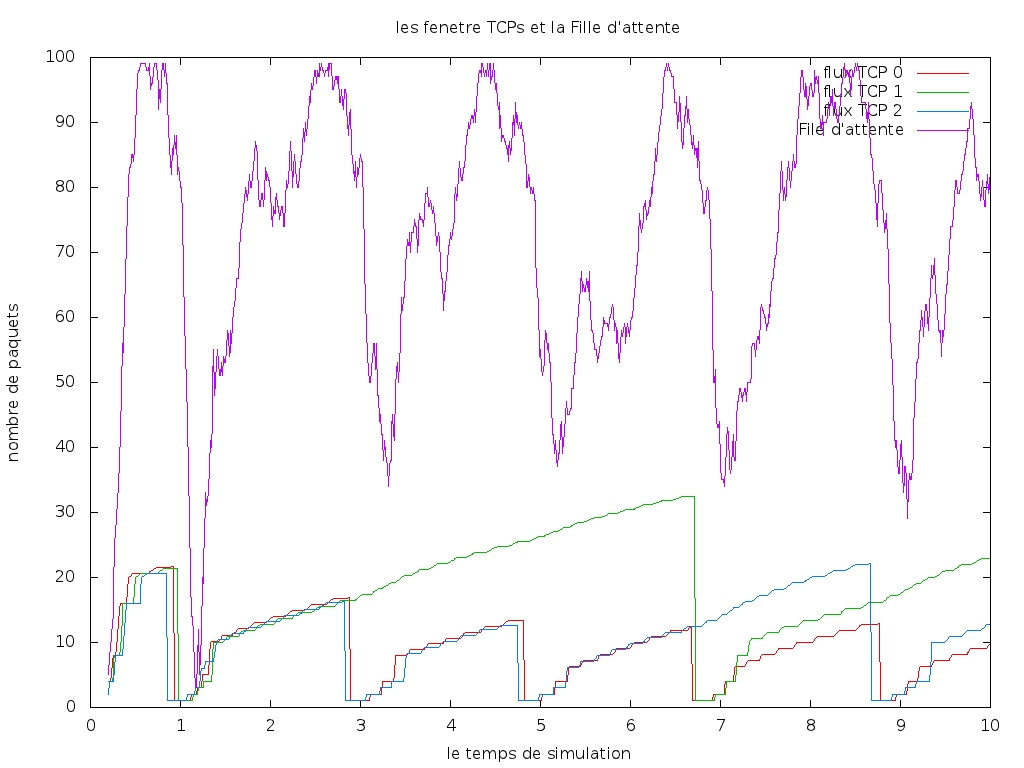
\includegraphics[width=450px]{graphic/rate75on10off5.png}
		\caption{le débit moyenne egal à 0.75Mb/s}
\end{figure}

\newpage
%%%%%%%%%%%%%%%%%%%%%%%%%%%%%%%%%%%%%%%%%%%%%%%%%%%%%%%%%%%%%%%%%%%%%%%%%
%%%%%%%%%%%%%%%%%%%%%%%%%%%%%%%%%%%%%%%%%%%%%%%%%%%%%%%%%%%%%%%%%%%%%%%%

\subsubsection*{périodes ON/OFF  :}
\paragraph*{}
   Maintenant, nous allons voir l'influance des périodes ON/OFF sur les résultat de simulation, et cela on diminuons c'est deux paramètres \\

	le tableau suivant représente les différents paramètres de la simulation NS2:
\begin{center}


\begin{tabular}{|c|c|}
\hline
 paramètre  & valeur \\ \hline
 
 Capacité de lien & 2Mbit/s(250000 o/s) \\ 
 Rate (Mbit/s) & 1.5 \\ 
 ON & 0.020  \\ 
 OFF & 0.010 \\ 
 Taille file d'att. & 100\\
\hline
\end{tabular}
\begin{tabular}{|c|c|c|}
\hline
 IdTCP  & Latence(s) & Taille de paquet (O) \\ \hline
 
 0 & 0.050 & 20936 b ( 2617 o)	 \\ 
 1 & 0.100 & 41872 b ( 5234 o)	 \\ 
 2 & 0.150 & 62808 b ( 7851 o)	 \\ 
 - & taille fene. & 20\\ 
&&\\ 
\hline
\end{tabular}\\
\end{center}

les résultats suivants sont obtenus avec ces paramètres à partir de la simulation ainsi que la formule: \\

\begin{tabular}{|l|c|c|c|c|c|c|c|}
\hline
 protocole & Taux Perte & Débit Moy.(O/S) Théorique & en Simulation (O/S) \\ \hline
 TCP0 & 0,057 &  133729,16 &  39836     \\
 TCP1 & 0,058 &  132571,31 &  49612     \\ 
 TCP2 & 0,061 &  129270,26 &  37132     \\ 
 UDP  & 0,069 &  187500     &  120540 \\ 
 \hline
 final perte & 0.068  & débit Moy. Sim. & 247120   \\ 
\hline
\end{tabular}

nous constatons une légère diminution de taux de perte (0.081 -> 0.068), ce qui presente l'influance de flux UDP sur la simulation.

la courbe suivante représente la taille des fenêtres TCPs et de la file d'attente en fonction de temps de simulations.  

%Figures 
\begin{figure}[h]
	\centering
		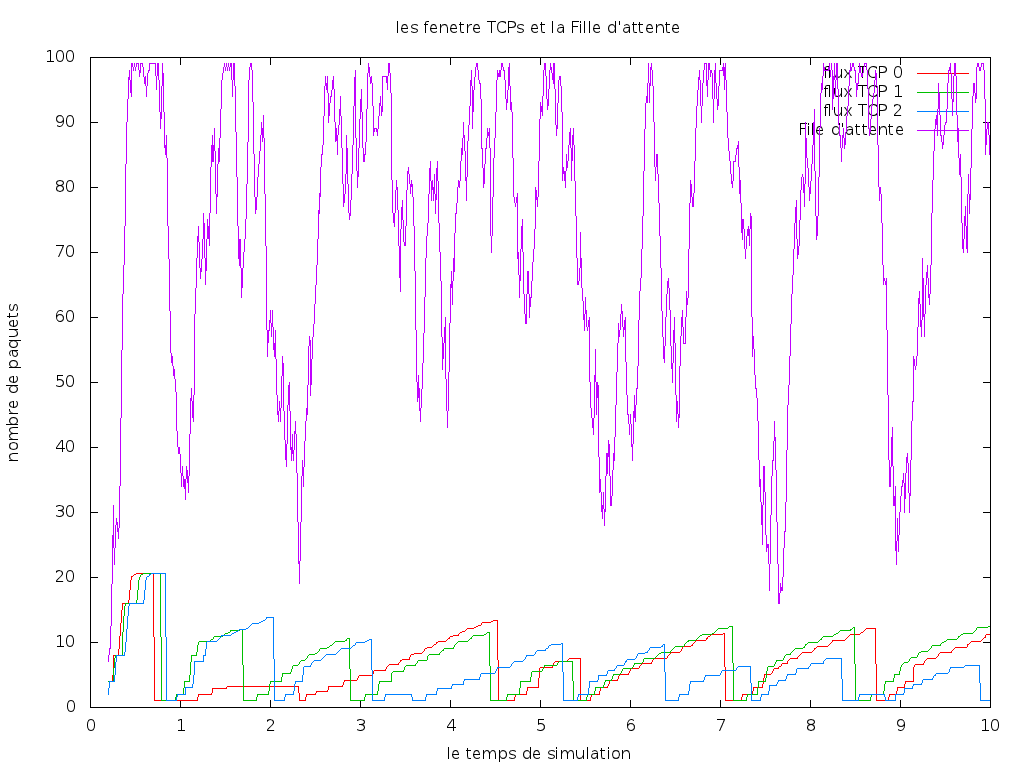
\includegraphics[width=450px]{graphic/rate1-5on20off10.png}
		\caption{période ON=20ms, OFF=10ms}
\end{figure}
Nous constatons une grande perturbation dans les résultats de la courbe, ce qui nous donne une relation entre ces deux paramètres (périodes ON/OFF) avec la taille de la file d'attente et les tailles des fenêtres TCPs. 

\newpage






%%%%%%%%%%%%%%%%%%%%%%%%%%%%%%%%%%%%%%%%%%%%%%%%%%%%%%%%%%%%%%%%%%%%%%%%%
%%%%%%%%%%%%%%%%%%%%%%%%%%%%%%%%%%%%%%%%%%%%%%%%%%%%%%%%%%%%%%%%%%%%%%%%

\subsubsection*{Le débit moyen et les périodes ON/OFF  :}
\paragraph*{}
   Maintenant, nous allons voir l'influance de changement(augmentation)  des trois paramètres vue précédament a la fois (débit moyen, périodes ON/OFF) sur le taux de perte ainsi sur le résultats de la simulation : \\
   \begin{center}
   

\begin{tabular}{|c|c|}
\hline
 paramètre  & valeur \\ \hline
 
 Capacité de lien & 2Mbit/s(250000 o/s) \\ 
 Rate (Mbit/s) & 2 \\ 
 ON & 0.100  \\ 
 OFF & 0.100 \\ 
 Taille file d'att. & 100\\
\hline
\end{tabular}
\begin{tabular}{|c|c|c|}
\hline
 IdTCP  & Latence(s) & Taille de paquet (O) \\ \hline
 
 0 & 0.050 & 20936 b ( 2617 o)	 \\ 
 1 & 0.100 & 41872 b ( 5234 o)	 \\ 
 2 & 0.150 & 62808 b ( 7851 o)	 \\ 
 - & taille fene. & 20\\ 
 &&\\
\hline
\end{tabular}\\
   \end{center}
	le tableau suivant représente les différents paramétres de la simulation NS2:\\

\begin{center}


\begin{tabular}{|l|c|c|c|c|c|c|c|}
\hline
 protocole & Taux Perte & Débit Moy.(O/S) Théorique & en Simulation (O/S) \\ \hline
 TCP0 & 0,16 &  79818,5 &  38900     \\
 TCP1 & 0,15 &  82436,19 &  30684     \\ 
 TCP2 & 0,18 &  75253,60 &  36404     \\ 
 UDP  & 0,099 & 250000     &  127008 \\ 
 \hline
 final perte & 0.11  & débit Moy. Sim. & 232996   \\ 
\hline
\end{tabular}\\
\end{center}
nous constatons une augmentation de taux de perte (0.081 -> 0.11), ce qui nous permet de conclure sur l'éxistance d'une relation d'ordre entre le flux UDP et le taux de perte.

la courbe suivante représente la taille des fenêtres TCPs et de la file d'attente en fonction de temps de simulations.  

%Figures 
\begin{figure}[h]
	\centering
		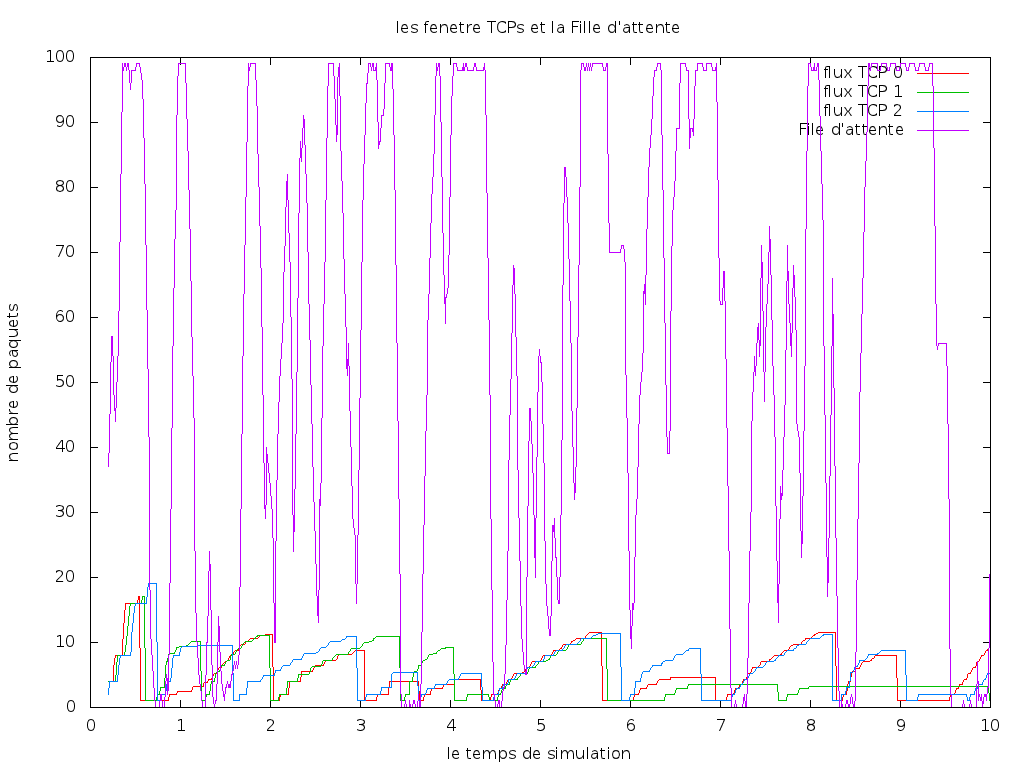
\includegraphics[width=450px]{graphic/rate2on100off100.png}
		\caption{le débit moyenne egal à 2Mb/s, ON=100ms, OFF=100ms}
\end{figure}

	Nous constatons une grande perturbation dans cette courbe, et cela nous confirme l'hypothese de liaison entre le flux UDP et la taille de la file d'attente ,ainsi celle des fenêtre TCPs.

\newpage


\section*{Conclusion} 
 Apres avoir éxcuter et analyser plusieurs simulations (8simulation) afin d'étudier le comportement des différents paramètres, et de définir la liaison entre ces paramètres, nous avons constaté des lien entre ces paramétre, soit avec une relation d'ordre, ou une relation inversé.
 
 	la graphique suivant represnte le taux de perte en fonction des différents changement de paramètres, et qui résume l'influance de chaque variable sur le paramètre le plus critique qui est le taux de perte.   

%Figures 
\begin{figure}[h]
	\centering
		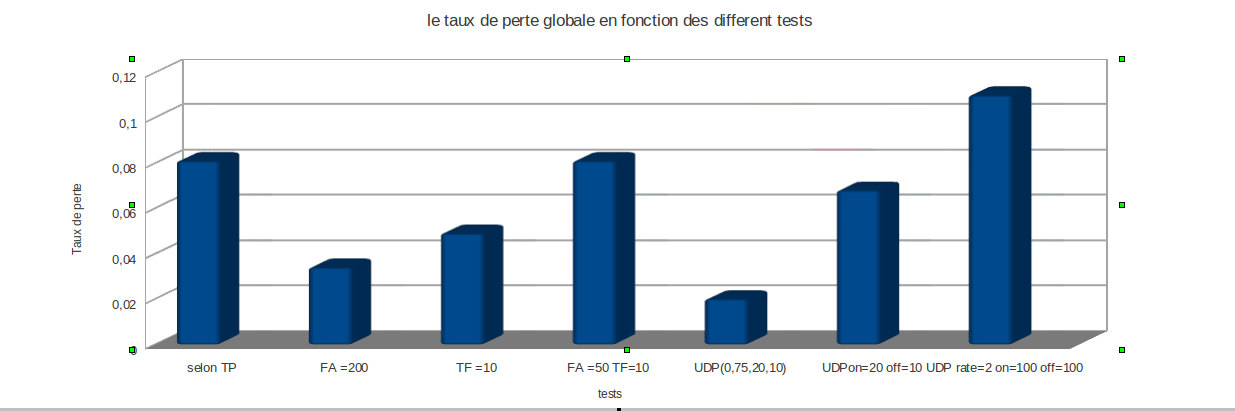
\includegraphics[width=400px]{graphic/conclu.png}
		\caption{le taux de perte globale dans les différents simulations}
\end{figure}
\newpage






















\chapter*{TP2}
\section*{Objectifs}
\begin{itemize}
 \item  Étudier un réseau de routeurs en anneau, soumis à différentes conditions de trafic.
 \item  Comparer les mesures avec les formules de la théorie.
 \item Analyser l’influence du trafic sur le taux de perte.
\end{itemize}

\section*{Topologie du reseau} 

Le réseau à étudier comporte six nœuds, numérotés de 1 à 6. Ces 6 noeuds forment un anneau.
Chaque noeud a une salle d’attente de capacité limitée à 100 paquets. Il y a six flots de paquets, dont
les origines et destinations sont connectées respectivement aux noeuds (1, 3), (2, 4), (3, 5), (4, 6), (5, 1) et
(6, 2). Le débit de la source connectée au nœud i est supposé égal à $\lambda_i = i \times \lambda_0$ paquets par seconde, où
$\lambda_0$ est un paramètre qui varie selon les expériences.
Les paquets seront générés par des sources UDP (dont on peut contrôler le débit plus facilement).
La taille des paquets sera de 1000 $octets$. Les liens entre nœuds auront une capacité de 106 $octets$ par
seconde. Le temps de propagation de chaque lien sera 50 $ms$.


%Fugure 2
	\begin{figure}[h]
	\centering
		\begin{tikzpicture}[auto,node distance=1.5cm,  semithick]
		 \tikzstyle{every node}=[draw,shape=circle,fill=white,minimum size=15pt, inner sep=0pt]
	
		  \node         (1)   		     {1};
  		  \node         (2) [ below of=1,xshift=15mm]    {2};
  		  \node         (3) [ below of=2]    {3};
  		  \node         (4) [ below of=3,xshift=-15mm]    {4};
  		 
  		  \node         (6) [ below of=1,xshift=-15mm]    {6};
		  \node         (5) [ below of=6]    {5};
		  \path(1) edge  (2);
		  \path(2) edge  (3);
		  \path(3) edge  (4);
		  \path(4) edge  (5);
		  \path(5) edge  (6);
		  \path(6) edge  (1);

		\end{tikzpicture}
		\caption{Topologie en anneau du reseau}
	\end{figure}

\paragraph{paramètres:} 
\section*{Code::Script}
\section*{Résultats} 

\end{document}
